% !Mode:: "TeX:UTF-8"
% Author: Zhengxi Tian
% Email: zhengxi.tian@hotmail.com

\chapter{实验结果与讨论}\label{ch:experiment}
本章从系统层面得分,句子层面得分和定性分析三个方面展示了实验的数据与结论。

\section{系统层面得分}\label{sec:system_scores}
图~\ref{tab:systemScoresAll}~展示了各个模型在不同数据集上测定的各种指标的系统层面得分,
加粗的得分是三个系统中的最优者。
从表中的数据来看,在LSDSCC上的最优模型是HRED,
在OpenSubtitles上的最优模型是VHRED,
在Ubuntu上的最优模型是HRED,它在9个指标中取得了最优,但是LSTM也在6个指标中取得了最优。

\begin{table}%
\centering%
\caption{不同数据集上的模型的各种指标得分}%
\label{tab:systemScoresAll}%
\begin{tabular}{|l|l|l|l|l|l|l|l|l|l|}%
\hline%
&\multicolumn{3}{c|}{LSDSCC}&\multicolumn{3}{c|}{OpenSubtitles}&\multicolumn{3}{c|}{Ubuntu}\\%
\hline%
&HRED&LSTM&VHRED&HRED&LSTM&VHRED&HRED&LSTM&VHRED\\%
\hline%
ADEM&2.6178&2.6127&2.6163&2.6228&2.6224&2.6219&2.6353&2.6381&2.635\\%
\hline%
BLEU{-}1&0.08&0.0726&0.0722&0.0672&0.0638&0.0753&0.1314&0.1303&0.1365\\%
\hline%
BLEU{-}2&0.0264&0.0181&0.0185&0.0171&0.0153&0.0264&0.0362&0.0345&0.0375\\%
\hline%
BLEU{-}3&0.0105&0.0052&0.0066&0.0062&0.0055&0.0146&0.009&0.007&0.0089\\%
\hline%
BLEU{-}4&0.0053&0.0&0.0028&0.0024&0.0022&0.01&0.0029&0.0018&0.0025\\%
\hline%
Distinct{-}1&0.9577&0.9441&0.9558&0.973&0.9714&0.9714&0.9074&0.9257&0.9113\\%
\hline%
Distinct{-}2&0.8541&0.8511&0.8497&0.8669&0.8594&0.8665&0.9013&0.8603&0.8968\\%
\hline%
Greedy&0.3303&0.3292&0.3267&0.3102&0.2998&0.3145&0.2775&0.2364&0.273\\%
\hline%
Average&0.5532&0.5467&0.5483&0.5453&0.5295&0.5485&0.574&0.5205&0.5655\\%
\hline%
Extrema&0.2841&0.2835&0.2814&0.3009&0.2929&0.3061&0.29&0.2663&0.2875\\%
\hline%
METEOR&0.0296&0.0258&0.0281&0.0248&0.0233&0.0271&0.1657&0.1635&0.166\\%
\hline%
ROUGE{-}1&0.108&0.083&0.0978&0.0784&0.075&0.0872&0.1644&0.1836&0.1683\\%
\hline%
ROUGE{-}2&0.0226&0.0049&0.0081&0.0053&0.0043&0.0107&0.0128&0.0143&0.0128\\%
\hline%
ROUGE{-}3&0.0057&0.0002&0.0035&0.0011&0.0009&0.0053&0.0007&0.0003&0.0005\\%
\hline%
ROUGE{-}4&0.0011&0.0&0.003&0.0002&0.0002&0.0038&0.0002&0.0&0.0001\\%
\hline%
ROUGE{-}L&0.0956&0.0681&0.0846&0.0742&0.0707&0.0826&0.1493&0.1722&0.1535\\%
\hline%
ROUGE{-}W&0.0792&0.0537&0.07&0.066&0.0629&0.0734&0.1205&0.1391&0.1236\\%
\hline%
PPL&32.5599&32.9229&37.7149&41.6392&34.2724&33.6867&39.178&46.4061&40.2641\\%
\hline%
\#words&13.1605&14.0067&12.3612&8.807&8.6394&8.7798&23.0646&16.4905&21.2449\\%
\hline%
\end{tabular}%
\end{table}

\section{句子层面得分}\label{sec:utterance_scores}
\subsection{指标的概率分布}\label{subsec:metric_distribution}
\begin{figure}[H]%
\centering%
\begin{subfigure}{0.3333333333333333\linewidth}%
\centering%
\includegraphics[width=\linewidth]{/home/cgsdfc/Metrics/Eval/data/v2/plot/distplot/lsdscc/hred/adem/plot.pdf}%
\end{subfigure}%
\begin{subfigure}{0.3333333333333333\linewidth}%
\centering%
\includegraphics[width=\linewidth]{/home/cgsdfc/Metrics/Eval/data/v2/plot/distplot/opensub/hred/adem/plot.pdf}%
\end{subfigure}%
\begin{subfigure}{0.3333333333333333\linewidth}%
\centering%
\includegraphics[width=\linewidth]{/home/cgsdfc/Metrics/Eval/data/v2/plot/distplot/ubuntu/hred/adem/plot.pdf}%
\end{subfigure}%
\newline%
\begin{subfigure}{0.3333333333333333\linewidth}%
\centering%
\includegraphics[width=\linewidth]{/home/cgsdfc/Metrics/Eval/data/v2/plot/distplot/lsdscc/lstm/adem/plot.pdf}%
\end{subfigure}%
\begin{subfigure}{0.3333333333333333\linewidth}%
\centering%
\includegraphics[width=\linewidth]{/home/cgsdfc/Metrics/Eval/data/v2/plot/distplot/opensub/lstm/adem/plot.pdf}%
\end{subfigure}%
\begin{subfigure}{0.3333333333333333\linewidth}%
\centering%
\includegraphics[width=\linewidth]{/home/cgsdfc/Metrics/Eval/data/v2/plot/distplot/ubuntu/lstm/adem/plot.pdf}%
\end{subfigure}%
\newline%
\begin{subfigure}{0.3333333333333333\linewidth}%
\centering%
\includegraphics[width=\linewidth]{/home/cgsdfc/Metrics/Eval/data/v2/plot/distplot/lsdscc/vhred/adem/plot.pdf}%
\end{subfigure}%
\begin{subfigure}{0.3333333333333333\linewidth}%
\centering%
\includegraphics[width=\linewidth]{/home/cgsdfc/Metrics/Eval/data/v2/plot/distplot/opensub/vhred/adem/plot.pdf}%
\end{subfigure}%
\begin{subfigure}{0.3333333333333333\linewidth}%
\centering%
\includegraphics[width=\linewidth]{/home/cgsdfc/Metrics/Eval/data/v2/plot/distplot/ubuntu/vhred/adem/plot.pdf}%
\end{subfigure}%
\caption{ADEM 在所有模型和数据集上的概率分布}%
\label{fig:ADEM{-}dist{-}all}%
\end{figure}
\begin{figure}[H]%
\centering%
\begin{subfigure}{0.3333333333333333\linewidth}%
\centering%
\includegraphics[width=\linewidth]{/home/cgsdfc/Metrics/Eval/data/v2/plot/distplot/lsdscc/hred/embedding_based_vector_average/plot.pdf}%
\end{subfigure}%
\begin{subfigure}{0.3333333333333333\linewidth}%
\centering%
\includegraphics[width=\linewidth]{/home/cgsdfc/Metrics/Eval/data/v2/plot/distplot/opensub/hred/embedding_based_vector_average/plot.pdf}%
\end{subfigure}%
\begin{subfigure}{0.3333333333333333\linewidth}%
\centering%
\includegraphics[width=\linewidth]{/home/cgsdfc/Metrics/Eval/data/v2/plot/distplot/ubuntu/hred/embedding_based_vector_average/plot.pdf}%
\end{subfigure}%
\newline%
\begin{subfigure}{0.3333333333333333\linewidth}%
\centering%
\includegraphics[width=\linewidth]{/home/cgsdfc/Metrics/Eval/data/v2/plot/distplot/lsdscc/lstm/embedding_based_vector_average/plot.pdf}%
\end{subfigure}%
\begin{subfigure}{0.3333333333333333\linewidth}%
\centering%
\includegraphics[width=\linewidth]{/home/cgsdfc/Metrics/Eval/data/v2/plot/distplot/opensub/lstm/embedding_based_vector_average/plot.pdf}%
\end{subfigure}%
\begin{subfigure}{0.3333333333333333\linewidth}%
\centering%
\includegraphics[width=\linewidth]{/home/cgsdfc/Metrics/Eval/data/v2/plot/distplot/ubuntu/lstm/embedding_based_vector_average/plot.pdf}%
\end{subfigure}%
\newline%
\begin{subfigure}{0.3333333333333333\linewidth}%
\centering%
\includegraphics[width=\linewidth]{/home/cgsdfc/Metrics/Eval/data/v2/plot/distplot/lsdscc/vhred/embedding_based_vector_average/plot.pdf}%
\end{subfigure}%
\begin{subfigure}{0.3333333333333333\linewidth}%
\centering%
\includegraphics[width=\linewidth]{/home/cgsdfc/Metrics/Eval/data/v2/plot/distplot/opensub/vhred/embedding_based_vector_average/plot.pdf}%
\end{subfigure}%
\begin{subfigure}{0.3333333333333333\linewidth}%
\centering%
\includegraphics[width=\linewidth]{/home/cgsdfc/Metrics/Eval/data/v2/plot/distplot/ubuntu/vhred/embedding_based_vector_average/plot.pdf}%
\end{subfigure}%
\caption{Average 在所有模型和数据集上的概率分布}%
\label{fig:Average{-}dist{-}all}%
\end{figure}

\subsection{不同指标的相关性分析}\label{subsec:metric_correlation}

\section{定性分析}\label{sec:qualitative_analysis}

\section{结果与讨论}\label{sec:result_and_discussion}

\section{本章小结}\label{sec:experiment_conclusion}
